% Template file for an a0 portrait poster.
% Written by Graeme, 2001-03 based on his SOC poster.
%
% See discussion and documentation at
% <http://www.astro.gla.ac.uk/users/norman/docs/posters/> 
%
%%%%%%%%%%%%%%%%%%%%%%%%%%%%%%%%%%%%%%%%
% Modified by Jozef Dobo\v{s} (c) 2011 % 
%%%%%%%%%%%%%%%%%%%%%%%%%%%%%%%%%%%%%%%%

\documentclass[a1,portrait]{a1poster}
% You might find the 'draft' option to a0 poster useful if you have
% lots of graphics, because they can take some time to process and
% display. (\documentclass[a0,draft]{a0poster})

\pagestyle{empty}
\usepackage{amsmath}
\setcounter{secnumdepth}{0}
\usepackage[absolute]{textpos}
\usepackage{wrapfig,times}
\usepackage{graphicx}
\usepackage{forloop}
\usepackage[margin=0cm]{geometry}
\usepackage{comment}
\usepackage[export]{adjustbox}
%\usepackage{framed,color}
\usepackage{tikz}
\usetikzlibrary{shapes,snakes}
\usepackage{setspace}
\usepackage{bm}
\usepackage[varg]{txfonts}
\usepackage{rotating}
\usepackage{physics}


\usepackage{color}
\usepackage[colorlinks, pdfborder={0 0 0}]{hyperref}
\definecolor{LinkColor}{rgb}{0.75, 0, 0}
\definecolor{CiteColor}{rgb}{0, 0.5, 0.5}
\definecolor{UrlColor}{rgb}{0, 0, 0.75}
\hypersetup{linkcolor=LinkColor}
\hypersetup{citecolor=CiteColor}
\hypersetup{urlcolor=UrlColor}
\DeclareMathAlphabet{\mathpzc}{OT1}{pzc}{m}{it}



%%%%%%%%%%
% Colors %
%%%%%%%%%%
\usepackage{color}
\definecolor{TitleColor}{rgb}{1,1,1} % white
\definecolor{BannerOneColor}{rgb}{0,0,0} % pitch black
\definecolor{BannerTwoColor}{rgb}{0.93,0.08,0.31} % pinky red
\definecolor{BannerThreeColor}{rgb}{0,0.27,0.48} % dark blue
\definecolor{BannerFourColor}{rgb}{0.33,0.19,0.098} % brown
\definecolor{BannerFiveColor}{rgb}{.93,0.,0.03} % some shade in red
\definecolor{BannerSixColor}{rgb}{0,0.27,0.42} % dark blue
\definecolor{BannerSevenColor}{rgb}{0.62,0.77,0.86} % sky blue
\definecolor{BannerEightColor}{rgb}{0.35,0.33,0.01} % military green
\definecolor{BannerNineColor}{rgb}{0.85,0.86,0.34} % lime green
\definecolor{BannerTenColor}{rgb}{0,0.66,0.80} % strong blue
\definecolor{BannerElevenColor}{rgb}{0.46,0,0.20} % maroon
\definecolor{BannerTwelveColor}{rgb}{0.37,0.32,0.44} % dark washed violet
\definecolor{BannerThirteenColor}{rgb}{0.79,0.84,0.65} % light washed green
\definecolor{BannerFourteenColor}{rgb}{0.57,0.64,0.27} % dark washed green
\definecolor{BannerFifteenColor}{rgb}{0.92,0.91,0.88} % unusable washed 
\definecolor{BannerSixteenColor}{rgb}{0.97,0.36,0.14} % strong orange
\definecolor{BannerSeventeenColor}{rgb}{0.97,0.61,0.19} % orange
\definecolor{BannerEighteenColor}{rgb}{0.99,0.76,0.11} % mustard yellow
\definecolor{BannerNineteenColor}{rgb}{0.79,0.76,0.73} % light gray-ish
\definecolor{BannerTwentyColor}{rgb}{0.63,0.58,0.54} % dark gray-ish

\definecolor{shadecolor}{rgb}{0.92,0.91,0.88} % unusable washed 
%%%%%%%%%%%%%%%%%%%%%%%%%%%%%%%%%%%%%%%%%%%%%%%%%%%%%%
% Only change here to affect all headings            %
\newcommand{\headingcolor}{\color{BannerElevenColor}} 
\newcommand{\FFe}{\mathrm{FF}_\mathrm{eff}}
\newcommand{\FF}{\mathrm{FF}}
\newcommand{\blambda}{\bm{\lambda}}
\newcommand{\rhosubopt}{\rho_\mathrm{subopt}}
\newcommand{\rhoopt}{\rho_\mathrm{opt}}
\renewcommand{\figurename}{Fig.}
\newcommand{\hlm}{\mathpzc{h}_{\ell m}}

\newcommand{\ajith}[1]{\textcolor{cyan}{\textit{Ajith:#1}}}


\newcommand{\Ms}{M_\mathrm{s}}
\newcommand{\Mf}{M_\mathrm{f}}
\newcommand{\Mo}{M_\mathrm{o}}
\newcommand{\mf}{m_\mathrm{f}}
\newcommand{\ms}{m_\mathrm{s}}
\newcommand{\mo}{m_\mathrm{o}}
\newcommand{\zs}{z_\mathrm{s}}
\newcommand{\zo}{z_\mathrm{o}}
\newcommand{\Gs}{G_\mathrm{s}}
\newcommand{\Gf}{G_\mathrm{f}}
\newcommand{\Go}{G_\mathrm{o}}
\newcommand{\dtgw}{\Delta t_\mathrm{GW}}
\newcommand{\dt}{\Delta t}
%%%%%%%%%%%%%%%%%%%%%%%%%%%%%%%%%%%%%%%%%%%%%%%%%%%%%%

% see documentation for a0poster class for the size options here
%\let\Textsize\normalsize
\let\Textsize\Large
\def\Head#1{\noindent\hbox to \hsize{\hfil{\LARGE \headingcolor #1}}\bigskip}
\def\LHead#1{\noindent{\LARGE \headingcolor #1}\smallskip}
\def\Authors#1{\noindent{\large#1}\smallskip}
\def\Subhead#1{\noindent{\large \headingcolor #1}}
\def\Title#1{\noindent{\huge #1}}

% define the color of the emphasis text here. Please use a text color 
% consistent with the color scheme of the poster 
\def\emphasis#1{{\large \color{BannerTwoColor} {#1}}}	

% Set up the grid
%
% Note that [0cm,0cm] is the margin round the edge of the page --
% it is _not_ the grid size. That is always defined as 
% PAGE_WIDTH/HGRID and PAGE_HEIGHT/VGRID. In this case we use
% 25 x 25. This gives us three wide columns for text (7 grid
% spacings) and four narrow columns (1 each) at each side of these 
% text columns
%
% Note however that texblocks can be positioned fractionally as well,
% so really any convenient grid size can be used.
%

% [margin, margin]{rows}{cols}
\TPGrid[0cm,0cm]{17}{25}  % 1 - 7 - 1 - 7 - 1 Columns


% Mess with these as you like
\parindent=0pt
%\parindent=1cm
\parskip=0.5\baselineskip
\linespread{1.1}

% abbreviations
\newcommand{\ddd}{\,\mathrm{d}}

\begin{document}

% Understanding textblocks is the key to being able to do a poster in
% LaTeX. In
%
%    \begin{textblock}{width}(x,y)
%    ...
%    \end{textblock}
%
% the first argument gives the block width in units of the grid
% cells specified above in \TPGrid; the second gives the (x,y)
% position on the grid, with the y axis pointing down.

%%%%%%%%%%%%%%
% Top Banner %
%%%%%%%%%%%%%%
% if you change this part, you can get matching color for headings
% in Colors section above


\begin{textblock}{25}(0,0)
%\includegraphics[width=\paperwidth]{banners/banner11.pdf}
\colorbox{BannerElevenColor}{\parbox[c][0.07\textwidth][c]{1.0\textwidth}{\rule{\linewidth}{0pt}}}
%\includegraphics[height=2.6in]{banners/banner11.pdf}
\end{textblock}




%%%%%%%%%%%%%%%%%%%%%%%%%%%%%%%%%%%%%%%%%%%%%%%%%%%%%%%%%%%%%%%%%%%%%%%%%
%%%%%%%%%%%%%%%%%%%%%%%%%%%%%%%%%% Title %%%%%%%%%%%%%%%%%%%%%%%%%%%%%%%%
%%%%%%%%%%%%%%%%%%%%%%%%%%%%%%%%%%%%%%%%%%%%%%%%%%%%%%%%%%%%%%%%%%%%%%%%%
\begin{textblock}{15}(0.75,0.1)	 % syntax: {colum_width} (x_coordinate, y_coordinate)
	{\color{TitleColor}
		
	\begin{center}
				\Title{Constraints on the time variation of the gravitational constant using gravitational-wave observations of binary neutron stars}
				
				{\Large [\ arXiv:2003.12832, accepted for publication in Phys. Rev. Lett. ]\ }
	\end{center}
	
	
	}
\end{textblock}


\begin{textblock}{23}(0.75,2.2)
\Authors{\textbf{Aditya Vijaykumar}$^1$, ~Shasvath J. Kapadia$^1$, ~Parameswaran Ajith$^{1,2}$} \\ 
\textit{$^1$ International Centre for Theoretical Sciences, Tata Institute of Fundamental Research, Bengaluru 560089, India} \\
\textit{$^{2}$ Canadian Institute for Advanced Research, CIFAR Azrieli Global Scholar, MaRS Centre, West Tower, 661 University Ave., Suite 505, Toronto, ON M5G 1M1, Canada} \\
\end{textblock}
%%%%%%%%%%%%%%%%%%%%%%%%%%%%%%%%%%%%%%%%%%%%%%%%%%%%%%%%%%%%%%%%%%%%%%%%%


%%%%%%%%%%%%%%%%%%%%%% An example text block %%%%%%%%%%%%%%%%%%%%%%%%%%%%
%%%%%%%%%%%%%%%%%%%%%%%%%%%%%%%%%%%%%%%%%%%%%%%%%%%%%%%%%%%%%%%%%%%%%%%%%

%%%%%%%%%%%%%%%%%%%%%%%%%%%%%%%%%%%%%%%%%%%%%%%%%%%%%%%%%%%%%%%%%%%%%%%%%
%%%%%%%%%%%%%%%%%%%%%% An example text block %%%%%%%%%%%%%%%%%%%%%%%%%%%%
%%%%%%%%%%%%%%%%%%%%%%%%%%%%%%%%%%%%%%%%%%%%%%%%%%%%%%%%%%%%%%%%%%%%%%%%%

\begin{textblock}{7}(1,3.8)	% syntax: {colum_width} (x_coordinate, y_coordinate) in inches
\LHead{Background}

The maximum and minimum allowed masses of neutron stars ($\ms^\mathrm{min,~max}$) at a particular cosmic epoch has a simple dependence on the value of $G=\Gs$ at that epoch,
\begin{equation}
\ms^\mathrm{min,~max} = m^\mathrm{min,~max} ~ (\Gs/\Go)^{-3/2}
\label{eq:m_max_min}
\end{equation}
where $\Go$ is the current value of $ G $, and $m^\mathrm{min,~max}$ is the current value of minimum and maximum mass for the neutron stars.

Let $ \mo $ be the measured (redshifted) mass. The template matching condition gives,
\begin{equation}
\mo = \frac{\Gs}{\Go} \, \left(\frac{1+\zs}{1+\zo}\right) \, \ms
\label{eq:m_obs_with_z}
\end{equation}
where $\zs$ is the true cosmological redshift of the source and $\zo$ is the estimated redshift, say, from an electromagnetic observation.

Using the above equations, we can derive the bounds within which the observed masses should lie,
\begin{equation}
\mo^\mathrm{max,~min} = m^\mathrm{max,~min}~(\Gs/\Go)^{-1/2}. 
\label{eq:m_obs_fn_Gf}
\end{equation}
That is, when $\Gs \neq \Go$, the allowed range of measured neutron star masses will be different from the range $m^\mathrm{min}$ --- $m^\mathrm{max}$. If $\Gs$ has a significant deviation from the current value $\Go$, the observed values of neutron star masses  would have gone out of the allowed range of neutron star masses. Hence such large deviations are ruled out by current GW observations. This is illustrated in Figure [\ref{fig:Gf_by_Go}].

\begin{textblock}{7}(1, 13)
	\LHead{Results}
	\begin{itemize}
		\item When {$\Gs \lesssim 4\times 10^{-3} \Go$ or when $\Gs \gtrsim 9 \Go$}, the observed mass range of the neutron stars in GW170817 will go out of the predicted mass range. Thus, the fractional deviation $\Delta G/\Go := (\Gs - \Go)/\Go$ in gravitational constant is constrained to be: $$\boxed{-0.996 \lesssim \Delta G/\Go \lesssim 8 }$$
		\item If we know the time $\Delta t$ elapsed between the merger and the GW observation, we can compute an average rate of change of the $G$ during this period: $\dot{G}/\Go \simeq \Delta G/(\Go \Delta t)$. For GW170817, we infer:
		$$\boxed{-7 \times 10^{-9}~\mathrm{yr}^{-1} \lesssim \dot{G}/\Go \lesssim 5 \times 10^{-8} ~\mathrm{yr}^{-1}}$$
	\end{itemize}
\end{textblock}

\begin{textblock}{7}(9,14)
	\LHead{Summary and Future Directions}
	
	\begin{itemize}
		\item Although our constraints are not as tight as the best available bounds from other measurements, they {sample a different cosmological epoch} that is not covered by other observations.
		\item Gravitational-wave observations sampling the extremes of the neutron star masses will further tighten these bounds.
		\item Additional detections of binary neutron stars would constrain the variation of G at different epochs. Projected constraints from third-generation GW detectors are shown in Figure [\ref{fig:gdot_plots}].
	\end{itemize}
\end{textblock}
\begin{comment}


\begin{figure}
	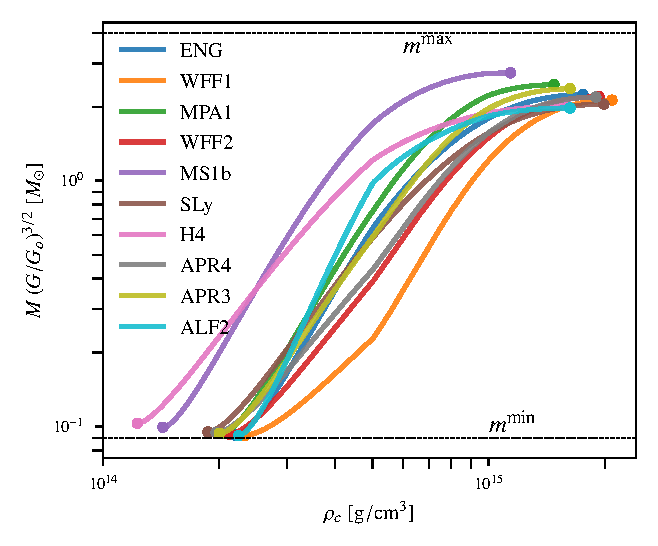
\includegraphics[width=1\linewidth]{mass_rhoc_curves.pdf}
	\caption{The mass of non-spinning neutron stars as a function of the central density $\rho_c$, computed numerically. We rescale the mass by $(G/\Go)^{3/2}$ where $G$ is the value of the gravitational constant used to solve the equations and $\Go = 6.67 \times 10^{-11}~\mathrm{m}^3\,\mathrm{kg}^{-1}\,\mathrm{s}^{-2}$ the current value of $G$. These relations between the rescaled mass and central density are independent of the value of $G$ used to compute the mass. The dots at the end of the curves correspond to the maximum/minimum mass supported by each equation of state. The horizontal dashed lines correspond to the maximum/minimum possible mass of neutron stars that we assume in this paper, independent of the equation of state.}
	\label{fig:M_R_plot}
\end{figure}
\end{comment}
\end{textblock}


\begin{textblock}{15}(1, 17.8)
	\begin{figure*}[t]
		\centering
		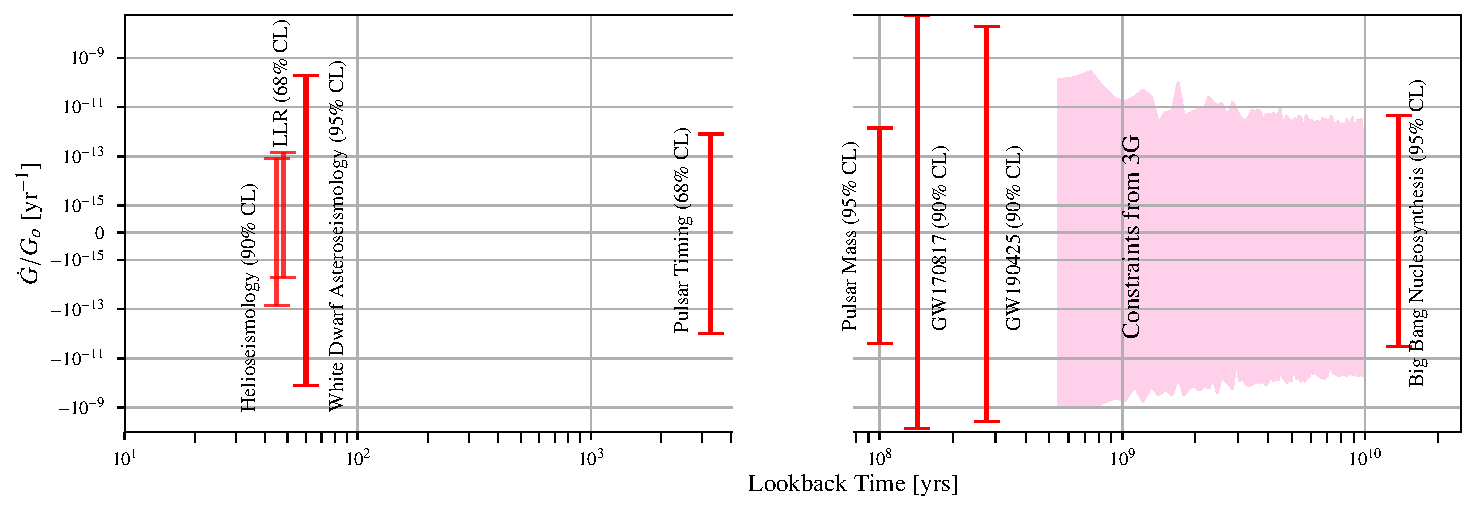
\includegraphics[width=0.95\linewidth]{gdot_over_cosmic_time.pdf}
		\caption{Comparison of the constraints on $\dot{G}/\Go$ obtained from various observations with confidence levels of the constraints indicated in brackets (LLR denotes constraints from lunar laser ranging). The horizontal axis shows the look back time. The constraints presented this paper are labeled as GW170817 and GW190425, while the expected constraints from 10 year of observations with third-generation (3G) GW detectors is shown by the pink band.}
		\label{fig:gdot_plots}
	\end{figure*}
\end{textblock}

\begin{textblock}{7}(9,3.5) % syntax: {colum_width} (x_coordinate, y_coordinate) in inches
	\LHead{}
\begin{wrapfigure}[7]{r}{24.5cm}
	 \fbox{%
		\begin{minipage}{\dimexpr24cm-\fboxsep-\fboxrule}
			\centering
	
	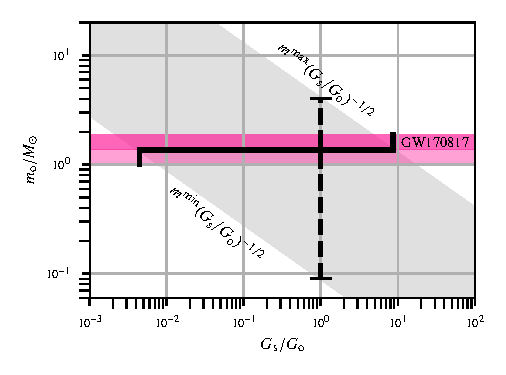
\includegraphics[width=1\linewidth]{GW170817_plot.pdf}
	\caption{
		%\begin{itemize}
		 \textit{The horizontal axis corresponds to the assumed value of $G=\Gs$ (in units of the current value $\Go$) at BNS merger epoch, and the vertical axis corresponds to the measured value of the neutron star mass $\mo$ (in units of $M_{\odot}$). The horizontal patches correspond to the measured value of the neutron star masses from GW170817  (90\% credible regions; the dark shade corresponds to primary mass while the light shade corresponds to secondary mass). The vertical dashed lines correspond to the theoretically allowed range of neutron star masses $m^\mathrm{min} - m^\mathrm{max}$ at the current epoch. The tilted gray regions show the allowed range of the observed neutron star mass (eq. [\ref{eq:m_obs_fn_Gf}]). The horizontal error bars show the constraints on $\Gs/\Go$ that we obtain by requiring that the measured values overlap with the theoretically allowed (gray) region.}
		%\end{itemize}
	}
	\label{fig:Gf_by_Go}
	\end{minipage}}
\end{wrapfigure}
\end{textblock}


%%%%%%%%%%%%%%%%%%%%%%%%%%%%%%%%%%%%%%%%%%%%%%%%%%%%%%%%%%%%%%%%%%%%%%%%%

%%%%%%%%%%%%%%%%%%%%%%%%%%%%%%%%%%%%%%%%%%%%%%%%%%%%%%%%%%%%%%%%%%%%%%%%%
%%%%%%%%%%%%%%%%%%%%%%%%%%%% Acknowledgments %%%%%%%%%%%%%%%%%%%%%%%%%%%%
%%%%%%%%%%%%%%%%%%%%%%%%%%%%%%%%%%%%%%%%%%%%%%%%%%%%%%%%%%%%%%%%%%%%%%%%%

%%%%%%%%%%%%%%%%%%%%%%%%%%%%%%%%%%%%%%%%%%%%%%%%%%%%%%%%%%%%%%%%%%%%%%%%%

\end{document}

